Au commencement du projet, un ensemble majeur de fonctionnalités - notamment la synchronisation, la résolution de conflits à l'aide de types de données répliqués sans conflit (CRDT), la gestion des clés cryptographiques et l'implémentation réseau - devait être réalisé par une entreprise externe. Cependant, pour diverses raisons, ce partenariat n'a pas abouti. Ceci a conduit à une réorientation majeure du projet : l'ensemble de ces fonctionnalités a dû être conçu et mis en oeuvre en interne.

C'est ainsi que le Decentralized Document Network (DDnet) a vu le jour. DDnet est un système de gestion de documents décentralisé axé sur le principe du "Local-First". Il permet de partager et de synchroniser des documents en temps réel entre plusieurs utilisateurs, le tout de manière sécurisée et chiffrée de bout en bout.

\section{Authentification et Gestion des Clés}

Le système conçu lors de ce projet identifie chaque utilisateur par sa clé publique. Les clés sont générées grâce à un système mnémonique inspiré de BIP39\footnote{\url{https://github.com/bitcoin/bips/blob/master/bip-0039.mediawiki}}, une norme facilitant la génération d'une clé privée à partir d'une phrase secrète, ce qui favorise la sauvegarde et la restauration des clés.

La réimplémentation du module npm \textit{bip39} a été nécessaire en raison de son incompatibilité avec les navigateurs, étant initialement conçu pour Node.js. Les fonctions et objets spécifiques à Node.js ont été substitués par leurs équivalents navigateur pour assurer la compatibilité. La taille du package a été significativement réduite, de 331 Ko à 57 Ko, grâce à cette réimplémentation, la rendant ainsi plus appropriée pour une utilisation navigateur. Le module réimplémenté est disponible sur npm sous le nom \textit{@describble/srp} (Secret Recovery Phrase)\footnote{\url{https://www.npmjs.com/package/@describble/srp}}.

Conformément au paradigme "Local-First", les clés privées sont stockées localement dans le navigateur de l'utilisateur. Cependant, le stockage en clair de ces clés serait problématique pour des raisons de sécurité. Par conséquent, les clés privées sont chiffrées à l'aide d'un mot de passe utilisateur. Ce mot de passe est d'abord dérivé via la fonction de dérivation PBKDF2\footnote{\url{https://en.wikipedia.org/wiki/PBKDF2}} avant d'être utilisé pour le chiffrement. Un sel aléatoire et un nombre d'itérations fixé à 10000 sont utilisés pour renforcer la sécurité de la dérivation. La clé dérivée est ensuite utilisée avec l'algorithme AES-GCM pour chiffrer la clé privée. Il convient de noter que le mot de passe n'est jamais stocké en clair ni transmis sur le réseau, il est seulement utilisé pour la dérivation de la clé de chiffrement.

J'ai également anticipé que plusieurs utilisateurs pourraient partager le même navigateur. Ainsi, pour préserver la confidentialité des données de chaque utilisateur, il est nécessaire de chiffrer les données spécifiques à chaque utilisateur. Cette mesure garantit que chaque utilisateur peut utiliser le même navigateur sans avoir accès aux données des autres.

La gestion des sessions est une partie délicate et complexe du système. Pour pouvoir signer ou chiffrer les données, le système doit avoir accès à la clé privée. Cependant, stocker cette clé en clair dans le navigateur serait inacceptable pour des raisons de sécurité. C'est pourquoi la clé privée en clair est uniquement stockée en mémoire. Cependant, la mémoire est effacée lors du rafraîchissement de la page. Pour pallier ce problème, j'ai décidé d'utiliser un Service Worker\footnote{\url{https://developer.mozilla.org/en-US/docs/Web/API/Service_Worker_API}}, dont le cycle de vie est indépendant de la page. Ainsi, la clé privée peut être stockée dans le worker et utilisée par la page. Toutefois, cette solution présente certaines limites, le cycle de vie d'un Service Worker étant indéterminé : il peut être détruit à tout moment par le navigateur, sans moyen de le prévoir.

\section{Connectivité et Serveur de Signalisation}

La capacité de synchroniser et partager des documents en temps réel constitue une fonctionnalité essentielle du système élaboré dans le cadre de ce projet. Cependant, pour respecter l'impératif de décentralisation, il est impossible de s'appuyer sur un serveur centralisé. WebRTC, un standard du W3C facilitant la communication en temps réel entre navigateurs, a donc été sélectionné pour établir une connexion pair à pair.

\subsection{Signalisation et Établissement de Connexion}

Néanmoins, pour que deux navigateurs puissent communiquer via WebRTC, ils doivent pouvoir se localiser sur le réseau. Cela nécessite l'intervention d'un serveur de signalisation, dont le rôle est de permettre aux navigateurs d'échanger les informations nécessaires pour établir une connexion directe. Une fois cette connexion établie, le serveur de signalisation n'intervient plus. Bien que des bibliothèques comme PeerJS\footnote{\url{https://peerjs.com/}} proposent un serveur de signalisation, elles ne sont pas compatibles avec le système d'authentification développé pour ce système. De ce fait, un serveur de signalisation personnalisé a été implémenté.

Le serveur de signalisation est un serveur Web qui recourt au protocole WebSocket, un protocole de communication bidirectionnel, pour instaurer une connexion persistante entre le client et le serveur. Pour l'implémentation du serveur de signalisation, Node.js a été choisi, en utilisant la bibliothèque ws\footnote{\url{https://www.npmjs.com/package/ws}} pour le protocole WebSocket. Bien que centralisé, le serveur de signalisation n'est pas un point de faiblesse du système. En effet, il ne traite pas de données sensibles et se contente de faciliter l'établissement d'une connexion directe entre deux clients. De plus, le serveur de signalisation est open-source et peut être auto-hébergé par les utilisateurs.

\subsection{Authentification par Serveur}

Le serveur de signalisation possède un module d'authentification, composé de trois classes distinctes : la classe Authenticator de base, la classe ServerAuthenticator, et la classe ClientAuthenticator. Ces classes sont conçues pour vérifier l'authenticité des connexions grâce à un mécanisme de poignée de main basé sur un défi-réponse cryptographique.

\subsubsection{Mécanisme de Défi-Réponse}

Le mécanisme de défi-réponse est une méthode pour prouver une identité en démontrant la connaissance d'un secret sans le révéler. Ici, un défi aléatoire est généré par le serveur et envoyé au client. Le client génère ensuite une réponse au défi en utilisant sa clé privée, qui peut être vérifiée avec la clé publique du client connue du serveur. Cela garantit l'identité du client, car seul le détenteur valide de la clé privée peut générer une réponse correcte.

Le processus d'authentification suit les étapes suivantes :

\begin{enumerate}
  \item Le serveur envoie un défi aléatoire au client.
  \item Le client reçoit le défi et crée une signature de réponse en utilisant sa clé privée.
  \item Le client renvoie la réponse signée au serveur.
  \item Le serveur vérifie la réponse en utilisant la clé publique du client.
  \item Si la vérification est réussie, le serveur reconnait le client comme authentifié. Sinon, il ferme la connexion.
\end{enumerate}

\begin{figure}[H]
  \begin{center}
    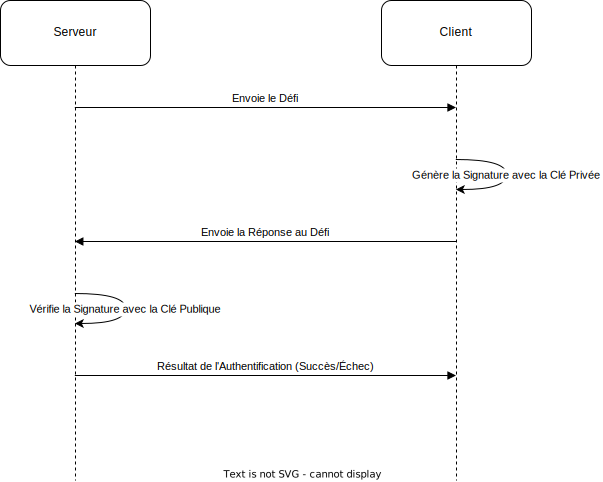
\includegraphics[width=0.75\textwidth]{\assetsdir/diagram-ddnet-auth.svg} % half of the text width
  \end{center}
  \caption[Mécanisme de Défi-Réponse]{Le diagramme représente le processus du mécanisme de défi-réponse utilisé pour l'authentification.}
\end{figure}

\subsection{Gestion des Connexions : Le Registre}

Le serveur de signalisation joue un rôle crucial dans le routage des messages entre les clients en maintenant un registre des clients et de leurs connexions actives. Ce registre est structuré comme un système de double registre imbriqué :

\begin{itemize}
  \item Le premier niveau du registre stocke les clés publiques des clients, chaque clé publique représentant un client unique.
  \item Le second niveau, imbriqué dans le premier, stocke les connexions associées à chaque clé publique. Chaque connexion est identifiée par un ID de client unique, qui est généré de manière aléatoire lors de l'établissement de la connexion.
\end{itemize}

Ce système de registre imbriqué offre un moyen efficace et organisé de stocker et de gérer les connexions. Il permet de facilement identifier et retracer toutes les connexions associées à un client spécifique, rendant ainsi le routage des messages plus efficace.

\begin{figure}[H]
  \begin{center}
    \includegraphics[width=0.75\textwidth]{\assetsdir/diagram-ddnet-registry.svg}
  \end{center}
  \caption[Registre et Connexions]{Le registre du serveur illustre les clés publiques des clients et leurs connexions associées.}
\end{figure}

En outre, le registre est également responsable de la gestion du cycle de vie des connexions. Lorsqu'une nouvelle connexion est établie, elle est automatiquement ajoutée au registre. De même, lorsque la connexion est fermée, le registre supprime cette connexion. Cela garantit que le registre reste toujours à jour, reflétant l'état actuel des connexions dans le réseau.

Ainsi, le registre facilite non seulement le routage des messages, mais contribue également à maintenir la santé globale et l'efficacité du réseau.

\subsection{Structure du Message}

La structure du message a été conçue en privilégiant la flexibilité et la sécurité. Dans cette perspective, chaque message comporte plusieurs champs qui lui permettent d'être adressé correctement, tout en maintenant l'intégrité des informations transmises.

\begin{listing}[H]
  \begin{minted}[breaklines,frame=none]{typescript}
type Message<TData> = {
  from: {
    publicKey: Uint8Array; // clé publique de l'expéditeur
    clientId: Uint8Array; // ID du client de l'expéditeur
  };
  to?: {
    publicKey: Uint8Array; // clé publique du destinataire
    clientId?: Uint8Array; // ID du client du destinataire (facultatif)
  };
  data: TData; // données contenues dans le message
};
\end{minted}
  \caption{Type Typescript de la structure d'un Message}
\end{listing}

\begin{itemize}
  \item Le champ \texttt{from} identifie l'expéditeur du message. Il comprend la clé publique de l'expéditeur, qui est unique pour chaque utilisateur, et l'ID du client de l'expéditeur, qui est unique pour chaque instance d'un utilisateur (par exemple, différentes fenêtres de navigateur ou différents appareils). Cela permet de retracer l'origine de chaque message.
  \item Le champ \texttt{to} est facultatif et identifie le destinataire du message. Si ce champ est spécifié, cela signifie que le message est privé et destiné à un utilisateur spécifique, déterminé par sa clé publique. En outre, si un ID de client est spécifié, le message est destiné à une instance spécifique de cet utilisateur. Si le champ \texttt{to} est omis, le message est considéré comme public et peut être reçu par n'importe quel utilisateur du réseau. Cette flexibilité permet une grande variété de types de communication, allant des messages directs à la diffusion publique.
  \item Le champ \texttt{data} contient les véritables données transportées par le message. Ces données sont génériques et peuvent être de n'importe quel type, permettant ainsi aux utilisateurs de transmettre une variété d'informations et d'instructions à travers le réseau.
\end{itemize}

\subsection{Transmission des Messages}

Les messages dans ce système peuvent être transmis de trois manières différentes en fonction du destinataire cible :

\begin{itemize}
  \item \textbf{Broadcast} : Un message est diffusé à tous les utilisateurs du réseau. C'est la méthode de transmission par défaut lorsque le champ `to` est omis.
  \item \textbf{Multicast} : Un message est envoyé à un utilisateur spécifique du réseau. C'est la méthode de transmission par défaut lorsque le champ `to` est spécifié, mais que le champ `clientId` est omis.
  \item \textbf{Unicast} : Un message est envoyé à une session spécifique d'un utilisateur dans le réseau. C'est la méthode de transmission par défaut lorsque le champ `to` est spécifié et que le champ `clientId` est spécifié.
\end{itemize}

La sécurité est une préoccupation majeure dans la transmission des messages dans ce système. Chaque message est signé numériquement par l'expéditeur, ce qui permet au serveur de vérifier son intégrité à la réception. Si le serveur détecte que le message a été altéré pendant la transmission, il le supprime immédiatement et arrête sa propagation.

La signature numérique garantit non seulement que le message provient bien de l'expéditeur déclaré, mais elle permet également de détecter tout changement ou corruption du contenu du message. Cela est crucial pour maintenir la confiance et la fiabilité du système de communication.

Voici un diagramme représentant la logique de routage :

\begin{figure}[H]
  \begin{center}
    \includegraphics[width=0.75\textwidth]{\assetsdir/diagram-ddnet-routing.svg}
  \end{center}
  \caption[Logique de Routage des Messages]{Schéma illustrant la logique de routage des messages dans le système.}
\end{figure}


\subsection{Chiffrement des Messages}

Le système chiffre automatiquement les messages si la clé publique du destinataire est spécifiée. Il implémente un protocole de transmission sécurisé, qui utilise la cryptographie pour maintenir la confidentialité et l'intégrité des messages. Les opérations cryptographiques spécifiques utilisées incluent :

\begin{itemize}
  \item \textbf{Diffie-Hellman sur courbes elliptiques (ECDH)} : Un protocole d'échange de clés qui permet à deux parties d'établir un secret partagé sur un canal non sécurisé. Ce secret partagé est généré en utilisant la clé privée de l'expéditeur et la clé publique du destinataire.
  \item \textbf{Fonction de dérivation de clés basée sur un mot de passe 2 (PBKDF2)} : Une fonction de dérivation de clés utilisée pour dériver une clé AES à partir du secret partagé obtenu lors de l'échange ECDH. Elle ajoute un sel pour la randomisation, offrant une résistance contre les attaques par dictionnaire.
  \item \textbf{Advanced Encryption Standard - Galois/Counter Mode (AES-GCM)} : Cet algorithme de chiffrement symétrique utilise la clé AES dérivée pour chiffrer le message, garantissant ainsi que seul le destinataire prévu peut le déchiffrer et le lire. L'AES-GCM assure à la fois la confidentialité et l'intégrité des données.
  \item \textbf{Algorithme de signature numérique sur courbes elliptiques (ECDSA) avec la courbe secp256k1} : Après que le message a été chiffré, il est signé en utilisant la clé privée de l'expéditeur. La signature permet de vérifier l'authenticité de l'expéditeur et confirme que le message n'a pas été altéré pendant la transmission.
\end{itemize}

Ce protocole assure une communication sécurisée et confidentielle, où seuls les destinataires prévus peuvent déchiffrer et lire le message.
Il vérifie également l'authenticité de l'expéditeur et garantit l'intégrité du message.

\section{Documents}

\subsection{En-tête du Document \label{doc_header}}

L'en-tête du document encapsule les métadonnées cruciales pour chaque document.
Ces métadonnées incluent des éléments tels que l'identifiant unique (ID) du document, la clé publique du propriétaire du document (servant de preuve de propriété), la liste des identifiants de clients autorisés à accéder au document, un objet avec des metadonnées arbitraires et le numéro de version actuel de l'en-tête. Un champ de signature supplémentaire, signé par le propriétaire du document, confirme l'authenticité et l'intégrité des données contenues dans l'en-tête.

\setlength{\extrarowheight}{2pt}

\begin{table}[h]
  \begin{center}
    \caption{Structure de l'en-tête du document.}
    \begin{tabularx}{\textwidth}{|c|c|X|}
      \hline
      \rowcolor{gray!20}
      \textbf{Propriété} & \textbf{Type}         & \textbf{Description}                                                                                 \\
      \hline
      id                 & \texttt{Uint8Array}   & Identifiant unique pour le document, généré en utilisant UUID v4 sous sa forme binaire sur 128 bits. \\
      \hline
      owner              & \texttt{Uint8Array}   & Clé publique du propriétaire du document.                                                            \\
      \hline
      allowedClients     & \texttt{Uint8Array[]} & Liste des identifiants de clients autorisés à accéder au document.                                   \\
      \hline
      metadata           & \texttt{any}          & Métadonnées supplémentaires.                                                                         \\
      \hline
      version            & \texttt{number}       & Version actuelle de l'en-tête.                                                                       \\
      \hline
      signature          & \texttt{Uint8Array}   & Signature de l'en-tête, signée par le propriétaire.                                                  \\
      \hline
    \end{tabularx}
  \end{center}
\end{table}



Le numéro de version joue un rôle essentiel dans la gestion du document. Chaque fois que l'en-tête du document est mis à jour, le numéro de version s'incrémente. Ce mécanisme assure un état de données cohérent et à jour à travers tout le réseau DDnet.

L'en-tête du document est conçu de manière immuable. Chaque fois qu'une mise à jour est apportée, une nouvelle instance de l'en-tête est créée. Cela garantit que l'en-tête du document ne peut pas être modifié une fois qu'il a été créé, ajoutant ainsi une couche de sécurité supplémentaire.

\subsection{Données du Document}

Les données du Document sont gérées à l'aide des types de données répliquées sans conflit (CRDT). Les CRDT sont des structures de données qui permettent à plusieurs répliques d'être mises à jour indépendamment et simultanément sans coordination entre elles. Les répliques peuvent ensuite être fusionnées sans conflits.
Comme mentionné précédemment, la gestion des données du document est effectuée par le package Automerge.

\subsection{Choix de la librairie de gestion de données répliquées sans conflit (CRDT)}

L'une des principales fonctionnalités du système DDnet est la synchronisation automatique et transparente des documents. Ce souci de simplicité d'utilisation ne doit pas compromettre la robustesse et la fiabilité du système. Dans cette optique, le choix de la librairie de gestion de données répliquées sans conflit (CRDT) est crucial.

Diverses librairies CRDT ont été examinées pour satisfaire à ces exigences. Yjs, par exemple, est une librairie CRDT bien connue. Cependant, Yjs a été écarté en raison de sa conception spécifique. En effet, Yjs crée ses propres structures de données et classes, ce qui pourrait rendre le projet DDnet excessivement dépendant de cette librairie et réduire sa modularité.

C'est finalement Automerge qui a été choisi. Cette librairie CRDT offre un degré élevé de modularité. Contrairement à Yjs, Automerge utilise des structures de données plus standard, telles que les tableaux et les objets JavaScript, ce qui facilite leur manipulation et leur intégration au projet.

Automerge se distingue techniquement par sa gestion des modifications. En effet, bien qu'Automerge reste complètement immuable, il utilise un système de proxy pour détecter les modifications. Cela est illustré dans l'exemple de code suivant :

\begin{listing}[H]
  \begin{minted}[breaklines,frame=none]{typescript}
type DocData = {
pets: Array<{name: string, type: string}>
}

// Création d'un document Automerge vide
let doc = automerge.init<DocData>()

// Modification du document
doc = automerge.change(doc, state => {
state.pets = [];
state.pets.push({name: "Lassie", type: "dog"});
state.pets.push({name: "Garfield", type: "cat"});
})

// Récupération des données du document
const pets = doc.pets
/*
pets = [
{name: "Lassie", type: "dog"},
{name: "Garfield", type: "cat"}
]
*/
\end{minted}
  \caption{Exemple de manipulation d'un document Automerge}
\end{listing}

Automerge utilise une fonction change où les modifications sont appliquées directement au document. Le document agit en tant que proxy pour détecter et enregistrer les modifications, tout en restant immuable. Les fonctions change renvoient une nouvelle instance du document avec les modifications intégrées, ce qui permet de conserver l'immuabilité du document tout en facilitant sa manipulation.

Un autre point important à noter est la fusion des documents avec Automerge. En fait, il est possible de fusionner deux documents ensemble, ce qui permet de garder les données à jour et cohérentes sur différents appareils ou sessions. Par exemple :

\begin{listing}[H]
  \begin{minted}[breaklines,frame=none]{typescript}
let doc2 = Automerge.init<DocData>()
doc2 = Automerge.merge(doc2, doc1)
  \end{minted}
  \caption{Exemple de fusion de deux documents Automerge}
\end{listing}

En ce qui concerne la persistance des données, Automerge fournit un mécanisme de sauvegarde au format binaire\cite{BinaryDocumentFormat}. Ce format est compact et optimisé pour le stockage, comme le montre l'exemple suivant :
\begin{listing}[H]
  \begin{minted}[breaklines,frame=none]{typescript}
let binary = Automerge.save(doc1)
let doc2 = Automerge.load(binary)
  \end{minted}
  \caption{Exemple de sauvegarde et chargement d'un document Automerge}
\end{listing}

Pour plus d'informations, consultez la documentation d'Automerge\footnote{\url{https://automerge.org}}.


\subsection{Sécurité des documents}

La sécurité des documents repose sur plusieurs mécanismes intégrés à leur conception. Le premier est l'utilisation d'une adresse unique pour chaque document. Cette adresse est générée en utilisant une fonction de hachage cryptographique, plus précisément SHA-256.

Pour obtenir cette adresse unique, la fonction de hachage SHA-256 est appliquée à la concaténation de l'identifiant unique du document et de la clé publique du propriétaire. Soit $id$ l'identifiant unique du document et $owner$ la clé publique du propriétaire, alors l'adresse du document est calculée comme suit :

\begin{equation}
  \text{Adresse du Document} = \text{SHA-256}(id | owner)
\end{equation}

La concaténation de $id$ et $owner$ est notée par "$|$". L'objectif de cette opération est double. D'abord, elle garantit l'unicité de l'adresse du document. De plus, elle permet de lier de manière intrinsèque l'adresse du document à la clé publique du propriétaire. Si une adresse ne correspond pas à la clé publique du propriétaire lors de la vérification, cela signifie que l'adresse a été altérée.

\subsection{Contrôle d'accès au document}

La gestion des documents au sein de DDnet repose sur deux piliers : le registre des documents, qui fait office de cache, et la persistance des documents.

\section{Cache et Persistance des Documents}

La gestion des documents au sein de DDnet repose sur deux piliers : le registre des documents, qui fait office de cache, et la persistance des documents.

\subsection{Registre des Documents}

Le registre des documents fonctionne comme un espace de stockage en mémoire, qui accueille les instances de documents actuellement utilisées ou récemment consultées. Cette caractéristique optimise l'efficacité du système, en fournissant un accès rapide aux documents tout en minimisant la sollicitation constante du système de persistance.

\subsection{Persistance des Documents}

La persistance des documents assure leur sauvegarde à long terme. Grâce à sa modularité, le système peut adopter plusieurs types de stockage. De plus, il est possible de créer des fournisseurs de persistance personnalisés pour étendre le système de persistance. Actuellement, quelques fournisseurs de persistance sont disponibles, comme décrit ci-dessous.

\subsubsection{IndexDB}

Pour le stockage côté navigateur, DDnet utilise principalement IndexDB. Contrairement à l'API LocalStorage qui est limitée en termes de type et de taille de données, IndexDB peut stocker des objets plus complexes, comme les ArrayBuffer. Cette capacité facilite la manipulation des structures de données complexes présentes dans DDnet. De plus, IndexDB n'est pas contraint par un quota de taille, ce qui le rend idéal pour des applications nécessitant un stockage de grande ampleur.

\subsubsection{Node FileSystem}

DDnet peut aussi utiliser le système de fichiers Node (Node FileSystem) pour le stockage local dans un environnement Node. Cette solution assure une persistance robuste, capable de répondre aux besoins du système.

\subsubsection{SecureProvider}

Afin de garantir la sécurité des données, DDnet propose le wrapper SecureProvider. Il peut être appliqué à n'importe quel fournisseur de stockage pour chiffrer les données avant leur sauvegarde. L'usage de ce wrapper nécessite une organisation spécifique du système de persistance. C'est pourquoi DDnet adopte une approche basée sur des namespaces. Ces derniers, pouvant correspondre à une clé publique par exemple, permettent au SecureProvider de déterminer le namespace à utiliser lors du chiffrement ou déchiffrement des données.

\subsection{Structure du Système de Persistance}

La persistance des données dans DDnet distingue les headers des documents de leurs données. Les headers sont stockés dans un namespace distinct, tandis que les données des documents sont stockées dans un autre namespace. Cette séparation optimise la gestion des documents, en fournissant un accès rapide aux headers tout en minimisant l'utilisation de la mémoire pour les données des documents.

DDnet gère intelligemment l'opération de sauvegarde. Lorsqu'un document est modifié, le système décide s'il est nécessaire d'effectuer une sauvegarde complète ou incrémentale en fonction du nombre de modifications depuis la dernière sauvegarde. Un mécanisme de limitation est également mis en place pour éviter des sauvegardes trop fréquentes pouvant ralentir l'application : les sauvegardes ne sont pas réalisées plus d'une fois toutes les 500 millisecondes.

\subsection{Chargement des Documents}

La procédure de chargement des documents dans DDnet est méticuleusement conçue pour être robuste et capable de s'adapter aux éventuels problèmes rencontrés pendant le processus de sauvegarde. Pour y parvenir, la procédure adopte une approche incrémentielle, qui se révèle particulièrement utile lorsque des segments de données, également appelés "chunks", sont corrompus ou inutilisables. Le processus de chargement suit plusieurs étapes distinctes:

\begin{enumerate}
  \item \textbf{Chargement Initial:} Dans un premier temps, DDnet tente de charger l'intégralité du document. Pour ce faire, le système récupère à la fois les données binaires et les chunks correspondants de l'identifiant du document à partir du système de stockage.
  \item \textbf{Échec du Chargement Initial:} Si le chargement complet du document échoue pour une raison quelconque, par exemple à cause d'un chunk corrompu, le système déclenche automatiquement une procédure de récupération.
  \item \textbf{Procédure de Récupération:} Cette procédure consiste à tenter de charger le document en éliminant progressivement un chunk à la fois à partir de la fin du document. Après chaque suppression de chunk, le système tente à nouveau de charger le document.
  \item \textbf{Sauvegarde Révisée:} Si le chargement du document réussit après avoir omis certains chunks, DDnet enregistre alors une nouvelle version du document sans les chunks omis, garantissant ainsi l'intégrité du document pour les futurs chargements.
  \item \textbf{Échec Total du Chargement:} Si, après avoir omis tous les chunks, le document ne peut toujours pas être chargé, alors DDnet génère une erreur. Cela peut indiquer un problème plus profond avec le document ou le système de stockage.
\end{enumerate}

Cette approche assure la robustesse du système en garantissant l'intégrité des documents, même en cas de problèmes survenant pendant le processus de sauvegarde. Elle veille à ce que chaque document reste fonctionnel et accessible, même en présence de segments de données défectueux ou inutilisables. Cette stratégie contribue à la résilience globale de DDnet, en permettant une récupération efficace des documents et en évitant la perte de données. Ainsi, les utilisateurs peuvent travailler en toute confiance, en sachant que la validité et l'accessibilité de leurs documents sont garanties, quelle que soit la situation.

\section{Accès aux documents}

Les documents dans le système DDnet sont gérés grâce à une série de processus qui facilitent leur création, récupération, mise à jour et suppression.

\subsection{Création de documents}

La création d'un document commence par l'utilisation de la clé privée de la session en cours pour générer et signer l'en-tête initial du document, comme décrit dans la section~\ref{doc_header}. Le document est ensuite enregistré dans le registre des documents. L'ajout du document au registre déclenche un événement système qui précise les clients autorisés à y accéder.

\subsection{Récupération de documents}

Pour récupérer un document, le système effectue d'abord une vérification dans le registre des documents. Si le document n'est pas dans le registre, le système cherche ensuite dans le stockage local. Si la recherche échoue également, une demande est envoyée au serveur de signalisation pour obtenir le document. Le système effectue alors une série de vérifications pour valider le document et les droits d'accès du client.

\subsection{Mise à jour de documents}

La mise à jour d'un document est gérée via le registre des documents. Que le document soit déjà présent dans le registre ou qu'il soit ajouté à ce dernier, la mise à jour déclenche un événement système. Cet événement entraîne une mise à jour du stockage local et une synchronisation avec les autres pairs.

\subsection{Suppression de documents}

Pour supprimer un document, le système effectue d'abord une vérification dans le registre des documents. Si le document est trouvé, il est supprimé du registre et du stockage local. Cette suppression déclenche un événement système.

\subsection{Partage de documents}

Le partage de documents implique la réception d'une demande de document via le serveur de signalisation. Le système vérifie ensuite la disponibilité du document et les droits d'accès du client demandeur. Si ces conditions sont remplies, le document est envoyé au client. Ce processus sécurisé utilise des clés privées et publiques pour assurer l'intégrité et la confidentialité des données.

En somme, le système d'accès aux documents de DDnet est un ensemble complexe de mécanismes qui garantissent non seulement une gestion efficace des documents, mais aussi la sécurité et la confidentialité des informations qu'ils contiennent.

\section{Le module de présence}
Le module de présence est un composant essentiel du système de partage de documents DDnet. Son rôle est de gérer les informations de présence, c'est-à-dire les données arbitraires échangées en temps réel entre les clients connectés à un document spécifique.

\subsection{Fonctionnement du module de présence}
Le module de présence s'appuie sur la connexion WebRTC existante pour communiquer les informations de présence. Grâce à cette infrastructure, les clients peuvent partager, recevoir et répondre aux informations de présence de tous les autres clients liés à un document.

Il est important de noter que les informations de présence sont éphémères : elles sont stockées uniquement en mémoire pendant la durée de la session. Lorsqu'un client se déconnecte, toutes ses informations de présence sont immédiatement supprimées. De plus, seuls les dernières données de présence envoyées par chaque client sont conservées, assurant ainsi la disponibilité des informations les plus récentes et pertinentes.

\subsection{Utilité du module de présence}
La flexibilité du module de présence lui permet d'implémenter une gamme de fonctionnalités collaboratives. Par exemple, il peut être utilisé pour afficher la position des curseurs des autres utilisateurs, permettant ainsi une conscience partagée de l'activité au sein du document. De même, un système de chat en temps réel peut être mis en place, où les messages sont considérés comme des informations de présence, assurant une communication en temps réel entre les utilisateurs.